  

%%%%%%%%%%%%%%Empieza la presentacion%%%%%%%%%%%%%%%%%%%%%%%%%%%%%%%%%%%%

%\begin{frame}
%\frametitle{Esquema}
 %   \tableofcontents
%\end{frame}


\subsection{Convoluci\'{o}n y filtrado}

\begin{frame}
\frametitle{Convoluci\'{o}n y filtrado}


\small

Definici\'{o}n convoluci\'{o}n para se\~{n}ales 1D x(n) de longitud finita $N$ :

\vspace{0.1cm}


\begin{itemize}

\item  $(x * y)(m)=\sum_{n=-\infty}^\infty x(n) h(m-n)=\sum_{n=0}^{N-1} x(n) h(m-n) $

\end{itemize}

\vspace{0.2cm}

\hrule

\vspace{0.2cm}


\small

\visible<2->{
Definici\'{o}n convoluci\'{o}n para se\~{n}ales 2D f(m,n) de tama\~{n}o $M * N$):

\vspace{0.1cm}

\begin{itemize}

\item $(f * h)(p,q))= \sum_{m=-\infty}^{\infty} \sum_{n=-\infty}^{\infty}  f(m,n) h(p-m,q-n)=$

\vspace{0.1cm}


\hspace{2.1cm}$=\sum_{m=0}^{M-1} \sum_{n=0}^{N-1}  f(m,n) h(p-m,q-n)$




\vspace{0.2cm}



\end{itemize}
}




\visible<3->{

Adem\'{a}s, si $h(m,n)$ es la respuesta de un sistema a la entrada impulso discreto $\delta(m,n)$, la respuesta del filtro a cualquier entrada la podemos calcular a trav\'{e}s de la convoluci\'{o}n.

\vspace{0.2cm}

}

\visible<4->{

Si tenemos $h(m,n)$  FIR, podremos calcular la respuesta con la orden \alert{conv2} o con la order \alert{filter2}.

\vspace{0.2cm}

}

\visible<4->{

Finalmente, la respuesta en frecuencia del filtro se puede obtener con la orden \alert{freqz2} (devuelve las frecuencias normalizadas)

\vspace{0.2cm}

}


\end{frame}


%%%%%%%%%
%%%%%%%%%



\begin{frame}
\frametitle{Ejemplos de convoluci\'{o}n y respuesta del filtro}

\small

\color{olivegreen} Ejemplo: \color{black} filtrado de una se\~{n}al 1D

\vspace{-0.2cm}

\begin{columns}[t]

\begin{column}{4.2cm}

\vspace{-0.7cm}


\lstinputlisting{./Matlab/Filtro1_1D.m}


\end{column}

\hspace{-0.3cm}\begin{column}{3.2cm}

\includegraphics[width=3.2cm,trim={0cm 0cm 0cm 0cm},clip,angle=0]{./Figures/F1D_Filter.eps}

\end{column}

\hspace{-0.4cm}\begin{column}{3.2cm}

\includegraphics[width=3.2cm,trim={0cm 0cm 0cm 0cm},clip,angle=0]{./Figures/F1D_Signals.eps}

\end{column}


\end{columns}

%%%%%%%%%%%%%%%%%%%%%

\vspace{-0.1cm}

\visible<2->{


\color{olivegreen} Ejemplo: \color{black} filtrado de una se\~{n}al 2D

\vspace{-0.2cm}

\begin{columns}[t]

\begin{column}{6cm}

\vspace{-0.7cm}


\lstinputlisting{./Matlab/Filtro1_2D.m}


\end{column}

\hspace{-0.4cm}\begin{column}{2cm}

\vspace{-1.3cm}

\includegraphics[width=2cm,trim={0cm 0cm 0cm 0cm},clip,angle=0]{./Figures/F2D_1.eps}

\includegraphics[width=2cm,trim={0cm 0cm 0cm 0cm},clip,angle=0]{./Figures/F2D_2.eps}

\end{column}

\hspace{-0.6cm}\begin{column}{1.5cm}

\vspace{-1.3cm}

\includegraphics[width=1.5cm,trim={0cm 0cm 0cm 0cm},clip,angle=0]{./Figures/F2D_3.eps}

\includegraphics[width=1.5cm,trim={0cm 0cm 0cm 0cm},clip,angle=0]{./Figures/F2D_4.eps}

\end{column}

\hspace{-0.6cm}\begin{column}{1.5cm}

\vspace{-1.3cm}

\includegraphics[width=1.5cm,trim={0cm 0cm 0cm 0cm},clip,angle=0]{./Figures/F2D_5.eps}

\includegraphics[width=1.5cm,trim={0cm 0cm 0cm 0cm},clip,angle=0]{./Figures/F2D_6.eps}

\end{column}


\end{columns}


}

\end{frame}

\begin{frame}
\frametitle{Filtros 2D FIR b\'{a}sicos}

\small

\begin{columns}[t]

\begin{column}{9cm}

\begin{itemize}
\item \alert{\textit{Filtro paso bajo}}: $h(m,n)=\frac{1}{MN}ones(M,N)$, promedia los valores en el entorno de la vecindad, suaviza los bordes y  elimina los detalles (alta frecuencia)


%\vspace{0.1cm}

\item \alert{\textit{Filtro paso alto (laplaciano)}}: 

$h(m,n)=\left [\begin{array}{ccc} -1 &-1 & -1 \\ -1 &8 &-1\\-1 &-1 &-1 \end{array}  \right ]$, elimina las bajas frecuencias y realza los bordes.


\end{itemize}

\end{column}

\begin{column}{3.5cm}

\includegraphics[width=3.0cm,trim={0cm 0cm 0cm 0cm},clip,angle=0]{./Figures/Filtro_Promedio.eps}

\vspace{0.2cm}

\includegraphics[width=3.0cm,trim={0cm 0cm 0cm 0cm},clip,angle=0]{./Figures/Filtro_Laplaciano.eps}

\end{column}

\end{columns}

\vspace{0.0cm}

\color{olivegreen}Ejemplo: \color{black} Filtrar una imagen con los dos filtros

\vspace{-0.8cm}

\begin{columns}[t]

\begin{column}{4.8cm}

\lstinputlisting{./Matlab/FiltrarEstanteria.m}

\end{column}

\begin{column}{2.0cm}

\vspace{0.8cm}

\includegraphics[width=2.0cm,trim={0cm 0cm 0cm 0cm},clip,angle=0]{./Figures/Libros1.eps}

\end{column}

\begin{column}{2.0cm}

\vspace{0.8cm}


\includegraphics[width=2.0cm,trim={0cm 0cm 0cm 0cm},clip,angle=0]{./Figures/Libros2.eps}

\end{column}

\begin{column}{2.0cm}

\vspace{0.8cm}


\includegraphics[width=2.0cm,trim={0cm 0cm 0cm 0cm},clip,angle=0]{./Figures/Libros3.eps}

\end{column}

\end{columns}


\end{frame}


\begin{frame}
\frametitle{Filtros 2D FIR proporcionados por Matlab}

\small

La orden \alert{h=fspecial(tipo,parametro)} permite general el nucleo de convoluci\'{o}n de diferentes filtros:

\footnotesize

\begin{itemize}

\item \alert{\textit{average}}: el filtro de promedio b\'{a}sico

\item \alert{\textit{disk}}: filtro circular paso b\'{a}sico

\item \alert{\textit{gaussian}}: filtro paso bajo gaussiano

\item \alert{\textit{laplacian}}: aproxima el operador laplaciano

\item \alert{\textit{log}}: laplaciano del filtro gaussiano

\item \alert{\textit{motion}}: aproxima el movimiento lineal de la camara

\item \alert{\textit{prewitt}}: filtro de enfatizado horizontal de Prewitt

\item \alert{\textit{sobel}}: filtro de enfatizado horizontal de Sobel

\end{itemize}

\small

\vspace{0.0cm}

\color{olivegreen}Ejemplo: \color{black} Filtrar una imagen con dos de los filtros

\vspace{-0.8cm}


\begin{columns}[t]

\begin{column}{4.8cm}

\lstinputlisting{./Matlab/FiltrarEstanteria2.m}

\end{column}

\begin{column}{2.0cm}

\vspace{0.8cm}

\includegraphics[width=2.0cm,trim={0cm 0cm 0cm 0cm},clip,angle=0]{./Figures/Libros1.eps}

\end{column}

\begin{column}{2.0cm}

\vspace{0.8cm}


\includegraphics[width=2.0cm,trim={0cm 0cm 0cm 0cm},clip,angle=0]{./Figures/Libros4.eps}

\end{column}

\begin{column}{2.0cm}

\vspace{0.8cm}

\includegraphics[width=2.0cm,trim={0cm 0cm 0cm 0cm},clip,angle=0]{./Figures/Libros5.eps}

\end{column}

\end{columns}


\end{frame}


\begin{frame}
\frametitle{Filtros 2D FIR Ideales}

\vspace{-0.3cm}

\scriptsize
\begin{columns}[t]
\begin{column}{5cm}

\centering

Filtro paso bajo

\vspace{0.2cm}

\includegraphics[width=4.5cm,trim={0cm 0cm 0cm 0cm},clip,angle=0]{./Figures/FiltroIdealPB.eps}

Filtro paso alto

\vspace{0.2cm}

\includegraphics[width=4.5cm,trim={0cm 0cm 0cm 0cm},clip,angle=0]{./Figures/FiltroIdealPA.eps}

\end{column}


%%%%%%%%%%%


\begin{column}{5cm}

\centering

Filtro paso banda

\vspace{0.2cm}

\includegraphics[width=4.5cm,trim={0cm 0cm 0cm 0cm},clip,angle=0]{./Figures/FiltroIdealPBanda.eps}

Filtro supresor banda

\vspace{0.2cm}

\includegraphics[width=4.5cm,trim={0cm 0cm 0cm 0cm},clip,angle=0]{./Figures/FiltroIdealSBanda.eps}

\end{column}


\end{columns}

\end{frame}


\begin{frame}
\frametitle{Filtros 2D FIR optimizando respuesta en frecuencia}

\small

Este procedimiento de dise\~{n}o de filtros FIR (que tambi\'{e}n se puede usar para se\~{n}ales 1D), consiste en encontrar la $h(m,n)$ que hace m\'{i}nimo

$e^2=\sum_{u=0}^M \sum_{v=0}^N |H(u,v)-H_{deseada}(u,v)|^2$

\vspace{0.2cm}

\visible<2->{
Debido a:
\begin{itemize}
\item La posibilidad de calcular matricialmente H(u,v) en funci\'{o}n de h(m,n) 
\item Ser un problema de minimos cuadrados
\end{itemize}

se puede calcular exactamente la $h(m,n)$ multiplicando/invirtiendo algunas matrices.}

\vspace{0.2cm}

\visible<3->{
En Matlab: \alert{$hmn=fsamp(Huv_{deseado})$}


}



\end{frame}



\begin{frame}
\frametitle{Ejemplo Filtros 2D FIR optimizando }

\small

\color{olivegreen}Ejemplo: \color{black} Obtener un filtro paso banda radial por el m\'{e}todo de optimizaci\'{o}n de la respuesta en frecuencia.


\vspace{-0.3cm}

\begin{columns}[t]
\begin{column}{6.5cm}




\lstinputlisting{./Matlab/FiltroOptimizado.m}

\end{column}

\begin{column}{4.0cm}

\vspace{0.5cm}

\includegraphics[width=4.0cm,trim={0cm 0cm 0cm 0cm},clip,angle=0]{./Figures/FiltroOptimizado.eps}

\end{column}


\end{columns}


\visible<2->{
\vspace{0.3cm}

\color{gray} Probar para distintos valores de N (tama\~{n}o del nucleo de convoluci\'{o}n) y comprobar que seg\'{u}n aumenta N es m\'{a}s f\'{a}cil obtener el comportamiento ideal. }



\end{frame}


